\documentclass[sokoban_generation_thesis.tex]{subfiles}

Autorzy wprowadzają metodę MCTS \cite{sok_mcts} jako autorską adaptację heurystyki \textit{Monte-Carlo Tree Search}. 

\subsection{Wprowadzenie}
\textit{Monte-Carlo Tree Search} jest heurystyką, której celem jest podejmowanie decyzji w~pewnych zadaniach sztucznej inteligencji. Metoda opiera swoje działanie na~przeszukiwaniu możliwych stanów zapisanych w~wierzchołkach drzewa i~losowym symulowaniu rozgrywek. Algorytmy z~grupy MCTS opierają się na~iteracyjnym rozbudowywaniu drzewa stanów przez sekwencyjne wykonanie czterech faz -- selekcji, ekspansji, symulacji i~propagacji wstecznej. Poszczególne fazy zostały zobrazowane na~rys.~\ref{rys:mcts_phases}.

\begin{figure}[h]
	\centering
	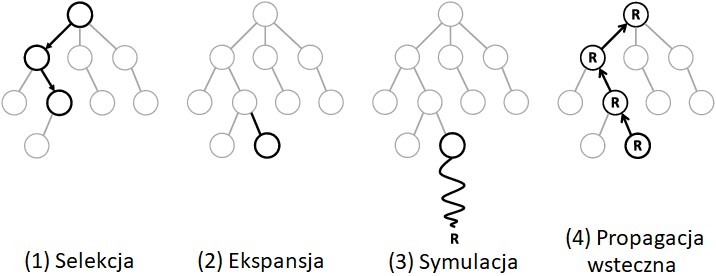
\includegraphics[width=0.8\textwidth]{mcts_phases_pl.png}
	\caption{Fazy MCTS, źródło: \cite{mctsanalysis}}
	\label{rys:mcts_phases}
\end{figure}

Faza selekcji w~heurystyce \textit{Monte-Carlo Tree Search} pozostawia dowolność w~wyborze liścia, który będzie eksploatowany w~kolejnych fazach. Oczywiście sposób wybierania liści w~kolejnych iteracjach jest krytyczny z~punktu widzenia eksploracji drzewa i~działania metody. W~literaturze opisywane są~różne podejścia, przykładowo UCB\_Minimal \cite{ucbminimal}, czy UCB-V \cite{ucbv}. Najbardziej powszechny i~użyty w~metodzie MCTS jest jednak wariant UCT \cite{uct_original}. Stara się on~zachować równowagę między eksploatacją bardziej obiecujących ruchów a~eksploracją tych rzadko odwiedzonych. Formuła UCB1, która odpowiada za~wyznaczenie najbardziej obiecującego wierzchołka w~fazie wyboru MCTS jest przedstawiona jako wyrażenie (\ref{eq:uct}). Indeks $i$ odnosi się do~liczby wykonanych przez algorytm iteracji. W~pierwszym składniku sumy wyrażenia (\ref{eq:uct}), licznik $w_i$ oznacza sumę wszystkich wypłat w~danym węźle, a~mianownik $n_i$ oznacza liczbę rozegranych symulacji. $N_i$ z~drugiego składnika sumy to~liczba symulacji rozegranych w~rodzicu danego węzła. Parametr eksploracji $c$ powinien zostać dobrany do~badanego problemu. Często dla funkcji wypłat o~wartościach w~przedziale $[0, 1]$ optymalnie jest przyjąć $c=\sqrt{2}$~\cite{uct_original}.

\begin{equation}\label{eq:uct}
	\frac{w_i}{n_i} + c~\sqrt{\frac{\ln N_i}{n_i}}
\end{equation}


\subsection{Opis metody}
Oryginalnie, algorytm \textit{Monte-Carlo Tree Search} uwzględnia istnienie dwóch graczy, dzieląc wierzchołki stanów na~te~uzyskane po~ruchu gracza pierwszego i~te~uzyskane po~ruchu gracza drugiego. Przechodząc w~trakcie fazy selekcji przez wierzchołki drzewa, odwraca się znak sumy wypłat gracza przeciwnego. Ta~operacja powoduje, że~iloraz wypłat i~odwiedzin przyjmuje wartości z~przedziału $[-1, 1]$. W~metodzie MCTS istnieje wyłącznie jeden gracz symulujący rozgrywkę, więc owy iloraz przyjmuje wartości nieujemne.

Jak wspomniano wyżej, metoda MCTS opiera swoje działanie na~symulowaniu zmodyfikowanej rozgrywki \textit{Sokoban}, która składa się z~dwóch faz. W~pierwszej gracz ma~do~wyboru trzy akcje: może usuwać przeszkody graniczące z~pustymi polami, stawiać pudła lub zamrozić planszę. Algorytm zaczyna pracę z~planszą w~pełni wypełnioną przeszkodami, więc zadaniem fazy pierwszej jest przygotowanie pustych pól. W~wyniku akcji zamrożenia, rozgrywka przechodzi do~fazy drugiej, w~której gracz prowadzi normalną rozgrywkę, poruszając się i~przesuwając pudła, do~momentu aż~zdecyduje się ją~zewaluować. Ewaluacja jest akcją, która kończy rozgrywkę i~dokonuje dodatkowych procesów czyszczenia w~celu uzyskania maksymalnie dobrej i~poprawnej planszy.

\subsection{Wypłaty} \label{subs:mcts_payoff}
Kluczowe dla metody MCTS jest dobranie funkcji oceniającej jakość generowanych poziomów (funkcji wypłaty). Jako że~\textit{Monte-Carlo Tree Search} opiera swoje działanie na~wielokrotnym symulowaniu rozgrywek, wyznaczanie wypłaty dla danego poziomu musi być mało kosztowne obliczeniowo. Autorzy metody zdecydowali się na~funkcję opisaną wzorem \ref{eq:mcts_metric} \cite{sok_mcts}, która jest sumą ważoną trzech metryk, podzieloną przez stałą $k$, dla znormalizowania wyniku. Wyrazy $w_b, w_c$ i~$w_n$ są~wagami dla odpowiednich metryk, opisanych poniżej. Wszystkie później prezentowane eksperymenty zostały przeprowadzone dla wartości $w_c=10$, $w_b=5$, $w_n=1$, $k=50$, zgodnie z~propozycją autorów metody. Mimo to, funkcja \ref{eq:mcts_metric} przyjmuje wartości większe niż $1$, do~czego nawiązują autorzy metody -- \textit{the parameter k~is~employed to~help normalize scores to~the range of~0 to~1, though some of~our top scoring puzzles can fall outside of~this range} \cite{sok_mcts}.

\begin{enumerate}
	\item Metryka pudeł 3~x~3 $P_b$ - liczba pól, która nie znajduje się w~bloku 3~x~3 przeszkód lub pustych pól. Zadaniem tej metryki jest nagrodzenie plansz, które nie zawierają bloków 3~x~3 tych samych pól, gdyż tego typu czynią plansze mniej skomplikowanymi.
	\item Metryka zagęszczenia $P_c$ - funkcja nagradzająca plansze o~długich ścieżkach między pudłami a~ich polami docelowymi.
	\item Metryka pudeł $P_n$ - liczba pudeł na~planszy.
\end{enumerate}

\begin{equation}\label{eq:mcts_metric}
	\frac{w_{b} P_{b}+w_{c} P_{c}+w_{n} P_n}{k}
\end{equation}